\documentclass[custom,grid]{flashcards}

\usepackage[T1]{fontenc}
\usepackage[danish]{babel}
\usepackage[pdftex]{graphicx}
\usepackage{amsfonts}
\usepackage{amsmath}
%\usepackage{MinionPro}
\usepackage{tikz}
\usetikzlibrary{calc,patterns,decorations.pathmorphing,decorations.markings,matrix,arrows}
\usepackage{mathtools}
\usepackage{bm}
\usepackage{mhchem}
\usepackage{chemmacros}
\usepackage{chemfig}
\usepackage{color}
\usepackage{modiagram}

\cardfrontstyle[\large]{headings}
\cardbackstyle{plain}
\setlength{\cardmargin}{0.8cm}

\begin{document}
% Fremstilling
% Struktur
% Reaktion
% Egenskab
% Anvendelse
% Trend
% Teori
\cardfrontfoot{Kapitel 9}
\begin{flashcard}[Trend]{Hvilken type bindinger danner grundstofferne i 5. hovedgruppe?}
Nitrogen og fosfor laver covalente bindinger. Arsen laver netv�rk-covalente bindinger. Antimon og bismuth laver metalliske bindinger.
\end{flashcard}

\begin{flashcard}[Trend]{Hvilken type bindinger danner grundstofferne i 2. periode?}
\begin{tabular}{ c | c | c | c | c | c | c | c }
\ce{Li} & \ce{Be} & \ce{B} & \ce{C} & \ce{N2} & \ce{O2} & \ce{F2} & \ce{Ne} \\ \hline
M & M & NC & NC & C & C & C & C
\end{tabular}\\ \vspace{7pt}
M = metallisk, NC = netv�rk covalent, C = covalent
\end{flashcard}

\begin{flashcard}[Trend]{Hvilken type bindinger danner grundstofferne i 3. periode?}
\begin{tabular}{ c | c | c | c | c | c | c | c }
\ce{Na} & \ce{Mg} & \ce{Al} & \ce{Si} & \ce{P4} & \ce{S8} & \ce{Cl2} & \ce{Ar} \\ \hline
M & M & M & NC & C & C & C & C
\end{tabular}\\ \vspace{7pt}
M = metallisk, NC = netv�rk covalent, C = covalent
\end{flashcard}

\begin{flashcard}[Trend]{Hvilken bindingstype er der tale om i de h�jeste flourider af grundstofferne i 2. periode?}
\begin{tabular}{ c | c | c | c | c | c }
\ce{LiF} & \ce{BeF2} & \ce{BF3} & \ce{CF4} & \ce{NF3} & \ce{OF2} \\ \hline
I & NC & C & C & C & C
\end{tabular}\\ \vspace{7pt}
I = ionisk, NC = netv�rk covalent, C = covalent
\end{flashcard}

\begin{flashcard}[Trend]{Hvilken bindingstype er der tale om i de h�jeste flourider af grundstofferne i 3. periode?}
\begin{tabular}{ c | c | c | c | c | c | c }
\ce{NaF} & \ce{MgF2} & \ce{AlF3} & \ce{SiF4} & \ce{PF5} & \ce{SF6} & \ce{ClF5} \\ \hline
I & I & NC & C & C & C & C
\end{tabular}\\ \vspace{7pt}
I = ionisk, NC = netv�rk covalent, C = covalent
\end{flashcard}

\begin{flashcard}[Trend]{Hvilken bindingstype er der tale om i de h�jeste oxider af grundstofferne i 2. periode?}
\begin{tabular}{ c | c | c | c | c | c }
\ce{Li2O} & \ce{BeO} & \ce{B2O3} & \ce{CO2} & \ce{N2O5} & \ce{F2O} \\ \hline
I & I & NC & C & C & C
\end{tabular}\\ \vspace{7pt}
I = ionisk, NC = netv�rk covalent, C = covalent
\end{flashcard}

\begin{flashcard}[Trend]{Hvilken bindingstype er der tale om i de h�jeste oxider af grundstofferne i 3. periode?}
\begin{tabular}{ c | c | c | c | c | c | c }
\ce{Na2O} & \ce{MgO} & \ce{Al2O3} & \ce{SiO2} & \ce{P4O10} & \ce{(SO3)3} & \ce{Cl2O7} \\ \hline
I & I & I & NC & C & C & C
\end{tabular}\\ \vspace{7pt}
I = ionisk, NC = netv�rk covalent, C = covalent
\end{flashcard}

\begin{flashcard}[Trend]{Hvilken bindingstype er der tale om i hydriderne af grundstofferne i 2. periode?}
\begin{tabular}{ c | c | c | c | c | c | c }
\ce{LiH} & \ce{(BeH2)_{$x$}} & \ce{B2H6} & \ce{CH4} & \ce{NH3} & \ce{H2O} & HF \\ \hline
I & NC & C & C & C & C & C
\end{tabular}\\ \vspace{7pt}
I = ionisk, NC = netv�rk covalent, C = covalent
\end{flashcard}

\begin{flashcard}[Trend]{Hvilken bindingstype er der tale om i hydriderne af grundstofferne i 3. periode?}
\begin{tabular}{ c | c | c | c | c | c | c }
\ce{NaH} & \ce{MgH2} & \ce{(AlH3)_{$x$}} & \ce{SiH4} & \ce{PH3} & \ce{H2S} & \ce{HCl} \\ \hline
I & I & NC & C & C & C & C
\end{tabular}\\ \vspace{7pt}
I = ionisk, NC = netv�rk covalent, C = covalent
\end{flashcard}

\begin{flashcard}[Trend]{Angiv syre/base egenskaberne af de h�jeste oxider af grundstofferne i 3. periode}
\begin{tabular}{ c | c | c | c | c | c | c }
\ce{Na2O} & \ce{MgO} & \ce{Al2O3} & \ce{SiO2} & \ce{P4O10} & \ce{(SO3)3} & \ce{Cl2O7} \\ \hline
B & B & A & S & S & S & S
\end{tabular}\\ \vspace{7pt}
B = basisk, S = sur, A = amfoter
\end{flashcard}

\begin{flashcard}[Trend]{Angiv syre/base egenskaberne af de h�jeste oxider af grundstofferne i 5. hovedgruppe}
\begin{tabular}{ c | c | c | c | c }
\ce{N2O5} & \ce{P4O10} & \ce{As2O3} & \ce{Sb2O3} & \ce{Bi2O3} \\ \hline
S & S & S & A & B
\end{tabular}\\ \vspace{7pt}
B = basisk, S = sur, A = amfoter
\end{flashcard}









\cardfrontfoot{Kapitel 10}
\begin{flashcard}[Fremstilling]{Hvorledes kan \ce{H2} fremstilles industrielt og i laboratoriet?}
Industrielt:\\ \ce{CH4 + H2O -> CO + 3 H2} \\ \ce{CO + H2O ->[\text{$\Delta$}] CO2 + H2} \\ \ce{K2CO3 + CO2 + H2O -> 2KHCO3} \\ \vspace{7pt}
I laboratoriet: \\ \ce{Zn(s) + 2HCl -> ZnCl2 + H2} \\ \vspace{7pt} samt ved elektrolyse i begge tilf�lde:\\
\ce{2 H2O + 2e- -> 2 OH- + H2}\\
\ce{6H2O -> 4H3O+ + O2 + 4e-}
\end{flashcard}

\begin{flashcard}[Trend]{Stiger eller falder reaktiviteten mellem \ce{H2} og halogenerne ned gennem 7. hovedgruppe?}
Reaktiviteten mellem dihydrogen og halogenerne falder ned gennem 7. hovedgruppe.
\end{flashcard}

\begin{flashcard}[Reaktion]{Beskriv hvordan \ce{H2} kan anvendes som reduktionsmiddel}
\ce{H2} kan anvendes p� organiske forbindelser:\\
\begin{align*}
\ce{H2\OX{rf1,\ox{-2,\ce{C}}}=\OX{rf2,\ox{-2,\ce{C}}}H2 + \OX{of1,\ox{0,\ce{H2}}} -> \OX{oe1,\ox{+1,\ce{H3}}}\OX{re1,\ox{-3,\ce{C}}}-\OX{re2,\ox{-3,\ce{C}}}\OX{oe2,\ce{H3}}}
\redox(of1,oe2){\small oxidation}
\redox(of1,oe1){}
\redox(rf1,re2)[][-1]{\small reduktion}
\redox(rf2,re1)[][-1]{}
\end{align*} \\ \vspace{7pt}
samt uorganiske, herunder metaloxider:\\
\begin{align*}
\ce{\OX{rf1,\ox{+2,\ce{Cu}}} O + \OX{of1,\ox{0,\ce{H2}}} -> \OX{re1,\ox{0,\ce{Cu}}} + \OX{oe1,\ox{+1,\ce{H2}}} O}
\redox(of1,oe1){\small oxidation}
\redox(rf1,re1)[][-1]{\small reduktion}
\end{align*}
\end{flashcard}

\begin{flashcard}[Trend]{Hvorledes kan hydriderne af grundstofferne i det periodiske system karakteriseres som henholdsvis ioniske, kovalente eller metalliske?}
Hydriderne af grundstofferne i 1. og 2. hovedgruppe kan karakteriseres som ioniske. \\
Hydriderne af overgangsmetallerne kan karakteriseres som metalliske. \\
Hydriderne af grundstofferne i 3. til 7. hovedgruppe kan karakteriseres som covalente.
\end{flashcard}

\begin{flashcard}[Egenskab]{Begrund hvorfor vands og flussyres kogepunkt er v�sentligt h�jere end forventet}
Intermolekyl�re hydrogenbindinger.
\end{flashcard}

\begin{flashcard}[Reaktion]{F�rdigg�r og afstem\\ \vspace{7pt}
\ce{H2 + Na -> NaH}\\
\ce{H2 + F2 -> HF}\\
\ce{H2 + O2 -> H2O}\\
\ce{H2 + N2 -> NH3}\\
\ce{H2 + CuO ->[\text{$\Delta$}] Cu}}

\ce{H2 + 2Na -> 2NaH}\\
\ce{H2 + F2 -> 2HF}\\
\ce{2H2 + O2 -> 2H2O}\\
\ce{3H2 + N2 -> 2NH3}\\
\ce{H2 + CuO ->[\text{$\Delta$}] Cu + H2O}
\end{flashcard}
\cardfrontfoot{Kapitel 11}

\begin{flashcard}[Reaktion]{Beskriv henholdsvis lithiums reaktion med atmosf�ren (oxygen og kuldioxid) samt alkalimetallernes reaktion med vand}

\ce{4Li + O2 -> 2Li2O}\\
\ce{Li2O + CO2 -> Li2CO3}\\ \vspace{7pt}
\ce{2K + 2H2O -> 2KOH + H2}\\
ligeledes for de andre.
\end{flashcard}

\begin{flashcard}[Egenskab]{Forklar hvorfor \ce{Li+} er exceptionel god til at koordinere vand}
\ce{Li+} har godt nok kun �n positiv ladning. Til geng�ld er Van der Walls radius af ionen relativt lille hvilket f�rer til en relativt h�j ladningst�thed (ladning pr. volumen). Det er ladningst�theden der afg�rer ionens evne til at koordinere vand.
\end{flashcard}

\begin{flashcard}[Egenskab]{Opskriv alkalimetallernes flammefarver}
\begin{tabular}{ l l }
Lithium & \color{red}R�d \\
Natrium & \color{yellow}Gul \\
Kalium & \color{violet}Lilla \\
Rubidium & \color{red}R�d-violet \\
Cesium & \color{blue}Bl�
\end{tabular}
\end{flashcard}

\begin{flashcard}[Egenskab]{Hvilken sammenh�ng er der mellem opl�seligheden af et salt, kationens radius og anionens radius?}
Kationer og anioner af nogenlunde samme st�rrelse vil have lettere ved at skabe et stabilt gitter (krystal, bundfald) end kationer og anioner med vidt forskellige st�rrelser. Derfor vil salte af ioner med stor st�rrelsesm�ssig forskel ofte v�re let opl�selige. Eksempelvis \ce{LiI}.
\end{flashcard}

\begin{flashcard}[Reaktion]{Opskriv reaktionen mellem nitrogen og et alkalimetal der har en r�d flammefarve og h�j ladningst�thed. Opskriv da produktets reaktion med vand.}
\ce{6Li + N2 -> 2Li3N} \\ \vspace{7pt}
\ce{Li3N + 3H2O -> NH3 + 3LiOH}
\end{flashcard}

\begin{flashcard}[Anvendelse]{Beskriv med ord og reaktionsskema hvorledes lithium indg�r i genopladelige Lithium-Ion batterier}
Anoden best�r af \ce{LiCoO2(s)} og katoden af grafit. Ved opladning bev�ger \ce{Li+} ioner sig fra anoden til katoden hvor de interkaleres i grafit katoden.\\ \vspace{7pt}
\ce{LiCoO2 -> Li_{($1-x$)}CoO2 + $x$Li+ + $x$e-} \\
\ce{C + $x$Li+ + $x$e- -> Li_{$x$}C} \\ \vspace{7pt}
Den modsatte reaktion finder sted ved afladning.
\end{flashcard}

\begin{flashcard}[Anvendelse]{Beskriv med reaktionsskema hvorledes lithium indg�r i ikke-genopladelige batterier}
De har alle lithiums ionisering (anodereaktionen) til f�lles: \ce{Li -> Li+ + e-}\\ \vspace{7pt}
Katodereaktionerne varierer batterityperne imellem. Her er tre forskellige batteritypers katodereaktion: \\
\ce{2SOCl2 + 4e- -> 4Cl- + SO2 + S} \\
\ce{SO2Cl2 + 2e- -> 2Cl- + SO2} \\
\ce{2SO2 + 2e- -> S2O4^{-2}}
\end{flashcard}

\begin{flashcard}[Fremstilling]{Opskriv hvordan titanium fremstilles industrielt}
\ce{TiCl4 + 4Na -> 4NaCl + Ti}
\end{flashcard}

\begin{flashcard}[Fremstilling]{Opskriv hvordan natrium og kalium fremstilles industrielt}
Natrium fremstilles ved elektrolyse af natriumchloridopl�sning \\ \vspace{7pt}
\ce{Na+ + e- -> Na} \\
\ce{2Cl- -> Cl2 + 2e-} \\ \vspace{7pt}
Kalium fremstilles ved f�lgende reaktion ved $850\,^{\circ}{\rm C}$ \\
\ce{Na(l) + KCl(l) -> K(g) + NaCl(l)}
\end{flashcard}

\begin{flashcard}[Fremstilling]{Opskriv hvordan natriumhydroxid fremstilles industrielt}
Elektrolyse af natriumchloridopl�sning \\ \vspace{7pt}
\ce{2H2O + 2e- -> H2 + 2OH-} \\
\ce{2Cl- -> Cl2 + 2e-} \\ \vspace{7pt}
De dannede hydroxid ioner er forhindret i at kommer i kontakt med chlorgassen af et diaphragm hvor natriumchloridopl�sningen kan passere.
\end{flashcard}

\begin{flashcard}[Reaktion]{Opskriv oxiderne af alkalimetallerne samt deres reaktion med vand}
\ce{Li2OH}, \ce{Na2O2}, \ce{KO2}. \\ \vspace{7pt}
\ce{Li2O + H2O -> 2LiOH} \\
\ce{Na2O2 + 2H2O -> 2NaOH + H2O2} \\
\ce{2KO2 + 2H2O -> 2KOH + H2O2 + O2}
\end{flashcard}

\begin{flashcard}[Anvendelse]{Beskriv med reaktionsligninger hvorledes \ce{KO2} kan bruges til at oplagre kuldioxid}
\ce{4KO2 + 2CO2 -> 2K2CO3 + 3O2} \\
\ce{K2CO3 + H2O + CO2 -> 2KHCO3}
\end{flashcard}

\begin{flashcard}[Generelt]{Er dioxid(2-)ionen para- eller diamagnetisk? Begrund med MO teori.}
$2p$ elektronerne danner f�lgende molekylorbitaler
\begin{MOdiagram}[style=fancy,labels,AO-width=8pt,labels-fs=\footnotesize]
\atom[\ce{O-}]{left}{2p={;pair,pair,up}}
\atom[\ce{O-}]{right}{2p={;pair,pair,up}}
\molecule[\ce{O2^{-2}}]{2pMO={1.3,.4;pair,pair,pair,pair,pair,}}
\end{MOdiagram}\\[-5pt]Diamagnetisk, ingen uparrede elektroner.
\end{flashcard}

\begin{flashcard}[Generelt]{Er dioxid(1-)ionen para- eller diamagnetisk? Begrund med MO teori.}
$2p$ elektronerne danner f�lgende molekylorbitaler
\begin{MOdiagram}[style=fancy,labels,AO-width=8pt,labels-fs=\footnotesize]
\atom[\ce{O-}]{left}{2p={;pair,pair,up}}
\atom[\ce{O-}]{right}{2p={;pair,up,up}}
\molecule[\ce{O2^{-2}}]{2pMO={1.3,.4;pair,pair,pair,pair,up,}}
\end{MOdiagram}\\[-5pt]Paramagnetisk, uparrede elektroner i $2\pi^{*}$.
\end{flashcard}

\begin{flashcard}[Reaktion]{Opskriv reaktionen mellem aluminium metal og hydroxidionen}
\ce{2Al + 2OH- + 6H2O -> 2[Al(OH)4]- + 3H2}
\end{flashcard}

\begin{flashcard}[Reaktion]{Hvad sker der med en natriumhydroxidopl�sning uden l�g?}
\ce{OH- + CO2 -> HCO3- }
\end{flashcard}

\begin{flashcard}[Reaktion]{Salte af alkalimetalionerne samt ammoniumionen er normalt letopl�selige. Som de eneste er alkalimetalionerne f.eks. letopl�selige som carbonater. Opskriv reaktioner hvorved \ce{Na+}, \ce{K+} og \ce{NH4+} kan bundf�ldes}
Natrium\\
\ce{Na+ + [Sb(OH)6]- -> Na[Sb(OH)6](s)} \\ \vspace{7pt}
Kalium og ammonium\\
\ce{3K+ + [Co(NO)6]^{3-} -> K3[Co(NO)6](s)}\\
\ce{3NH4+ + [Co(NO)6]^{3-} -> (NH4)3[Co(NO)6](s)}
\end{flashcard}

\begin{flashcard}[Anvendelse]{Beskriv med reaktionsskemaer hvorledes natriumbicarbonat anvendes i bagepulver}
Bagepulver best�r af \ce{NaHCO3} samt \ce{Ca(H2PO4)2}.\\ \vspace{7pt}
\ce{2NaHCO3 + Ca(H2PO4)2 ->[\text{$\Delta$}] NaHPO4 + CaHPO4 + 2CO2 + 2H2O}
\end{flashcard}

\begin{flashcard}[Reaktion]{Hvad sker der med natriumbicarbonat n�r det opvarmes?}
\ce{2NaHCO3 -> Na2CO3 + CO2 + H2O}
\end{flashcard}

\begin{flashcard}[Egenskab]{Beskriv med ord og reaktionsskema hvad der sker n�r et alkalimetal, i dette tilf�lde natrium,  opl�ses i ammoniak}
\ce{Na(s) -> Na+(ammoniak) + e^{-}(ammoniak)}\\
Opl�sningen vil have en dyb bl� farve n�r den er tynd og en bronze farve n�r det er koncentreret. Med tiden vil natrium reagere med ammoniak og danne natriumamid\\
\ce{2Na+ + 2NH3 + 2e- -> 2NaNH2 + H2}
\end{flashcard}

\begin{flashcard}[Fremstilling]{Hvordan findes kaliumchlorid i naturen og hvordan udvindes det?}
\ce{KCl} findes bl.a. som \ce{KMgCl3\cdot 6H2O} samt \ce{MgSO4\cdot H2O}. Udvindes v. 3 forskellige metoder.\\
\begin{itemize}
\item Udnyt forskellige opl�sligheder af saltene ved at opl�se dem. Energikr�vende at fordampe vand.
\item Opl�s i saltlage. Bl�s luft igennem. \ce{KCl} sidder fast p� boblernes overflade som opfanges.
\item Elektrostatisk proces. Mal krystaller til pulver og giv dem ladning via. friktion. De kan herefter adskilles.
\end{itemize}
\end{flashcard}

\begin{flashcard}[Fremstilling]{Fra hvilket mineral og hvordan udvindes \ce{Na2CO3}?}
Trona: \ce{Na2CO3\cdot NaHCO3 \cdot 2H2O}\\ \vspace{7pt}
Opvarmning, rekrystallisation, opvarmning\\
\ce{2Na2CO3\cdot NaHCO3 \cdot 2H2O ->[\text{$\Delta$}] 3Na2CO3 + 5H2O + CO2}\\
Natriumcarbonat genopl�ses hvorved faste urenheder filtreres fra. \ce{Na2CO3\cdot H2O} opn�s ved t�rring.\\
\ce{Na2CO3\cdot H2O ->[\text{$\Delta$}] Na2CO3 + H2O(g)}
\end{flashcard}

\begin{flashcard}[Fremstilling]{Beskriv hvorledes \ce{Na2CO3} kan fremstilles ud fra Solvay processen}
\ce{2NaCl + CaCO3 <=> Na2CO3 + CaCl2}
\end{flashcard}

\begin{flashcard}[Anvendelse]{Beskriv med reaktionsskema hvorledes \ce{Na2CO3} anvendes i produktionen af glas.}
\ce{Na2CO3 + $x$SiO2 ->[\text{$\Delta$}] Na2O\cdot $x$SiO2 + CO2 }
\end{flashcard}
\cardfrontfoot{Kapitel 12}

\begin{flashcard}[Teori]{Begrund at magnesium(II) har en mindre ionradius end natrium(I)}
Begge ioner har den samme elektronkonfiguration $1s^{2}2s^{2}2p^{6}$\\ \vspace{7pt}
Dog har magnesium �n proton mere end natrium. Det betyder, at magnesium kan ud�ve en st�rre tiltr�kkende kraft p� elektronerne s�ledes at de befinder sig t�ttere p� kernen.
\end{flashcard}

\begin{flashcard}[Reaktion]{Opskriv reaktionen mellem en (for det meste) intert gas og magnesium metal}
\ce{3Mg + N2 -> Mg3N2}
\end{flashcard}

\begin{flashcard}[Egenskab]{Angiv hvilke af jordalkalimetallerne der er opl�selige med \ce{CO3^{2-}}, \ce{PO4^{3-}}, \ce{SO4^{2-}} og \ce{OH-}}
\begin{tabular}{ r|c|c|c|c| }
 \multicolumn{1}{r}{}
  & \multicolumn{1}{c}{\ce{CO3^{2-}}}
  & \multicolumn{1}{c}{\ce{PO4^{3-}}}
  & \multicolumn{1}{c}{\ce{SO4^{2-}}}
  & \multicolumn{1}{c}{\ce{OH-}}
  
   \\
 \cline{2-5}
 \ce{Mg^{2+}}& & & Opl�selig & \\
 \cline{2-5}
 \ce{Ca^{2+}} & & & (Opl�selig) & (Opl�selig) \\
 \cline{2-5}
 \ce{Sr^{2+}} & & & & Opl�selig \\
 \cline{2-5}
 \ce{Ba^{2+}} & & & & Opl�selig \\
 \cline{2-5}
 \end{tabular}
\end{flashcard}

\begin{flashcard}[Reaktion]{Vis med reaktionsskema at berylliumoxid er amfotert}
\ce{BeO + 2H3O+ + H2O -> [Be(OH2)4]^{2+}}\\ \vspace{7pt}
\ce{BeO + 2OH- + H2O -> [Be(OH)4]^{2-}}
\end{flashcard}

\begin{flashcard}[Teori]{Begrund hvorfor beryllium har tendens til at danne covalente forbindelser}
Beryllium er relativt elektronegativ. Man kan forudsige bindingskarakter ud fra elektronegativitet. Et eksempel er \ce{BeCl2}. Forskellen mellem elektronegativitet for disse er $3.16-1.57=1.59$ hvilket svarer til en pol�r kovalent binding.
\end{flashcard}

\begin{flashcard}[Struktur]{Optegn strukturen af \ce{[Be(OH2)4]^{2+}}}
\schemestart
$\chemleft[\chemfig{Be(-[2]\ce{OH2})(-[5]\ce{H2O})(<[:-50]\ce{OH2})(<:[:-12]\ce{OH2})}\chemright]^{2+}$
\schemestop
\end{flashcard}

\begin{flashcard}[Fremstilling]{Hvordan findes magnesium i naturen?}
Magnesium findes i naturen som \ce{KMgCl3\cdot 6H2O}, \ce{CaMg(CO3)2} og \ce{MgSO4\cdot 7H2O}
\end{flashcard}

\begin{flashcard}[Reaktion]{Opskriv reaktion for forbr�nding af magnesium metal med oxygen henholdsvis carbondioxid}
\ce{2Mg + O2 -> 2MgO} \\ \vspace{7pt}
\ce{2Mg + CO2 -> 2MgO + C}
\end{flashcard}

\begin{flashcard}[Fremstilling]{Beskriv den industrielle fremstilling af magnesium}
\ce{Ca(OH)2 + Mg^{2+} -> Mg(OH2)(s) + Ca^{2+}} \\
\ce{Mg(OH)2 + 2HCl -> MgCl2(aq) + 2H2O} \\
Elektrolyse af \ce{MgCl2} giver \ce{Mg} ved katoden og chlorgas ved anoden. Chlorgas kan genbruges til at danne saltsyre.
\end{flashcard}

\begin{flashcard}[Reaktion]{Hvad sker der n�r \ce{CaCO3} opvarmes?}
\ce{CaCO3 -> CaO + CO2}
\end{flashcard}

\begin{flashcard}[Reaktion]{Opskriv hovedkomponenterne i klinker samt reaktionen hvorved cement h�rder}
Hovedkomponenterne i klinker er \ce{Ca3SiO5}, \ce{Ca3Al2O6} og \ce{Ca4Al2Fe2O10}.\\ \vspace{7pt}
\ce{2Ca3SiO5 + 7H2O -> Ca3Si2O7\cdot 4H2O + 3Ca(OH)2}\\
\ce{Ca(OH)2 + CO2 -> CaCO3 + H2O}
\end{flashcard}

\begin{flashcard}[Reaktion]{Opskriv den kemiske formel for gips og for det tilsvarende hemihydrat}
Gips: \ce{CaSO4\cdot 2H2O}\\ \vspace{7pt}
Tilsvarende hemihydrat: \ce{CaSO4\cdot $\frac{1}{2}$H2O}
\end{flashcard}

\begin{flashcard}[Fremstilling]{Opskriv reaktionen for dannelse af calciumcarbid}
\ce{CaO + 3C ->[\text{$\Delta$}] CaC2 + CO}
\end{flashcard}

\begin{flashcard}[Reaktion]{Opskriv calciumcarbids reaktion med vand henholdsvis nitrogen}
\ce{CaC2 + 2H2O -> Ca(OH)2 + C2H2}\\ \vspace{7pt}
\ce{CaC2 + N2 -> CaCN2 + C}
\end{flashcard}
\cardfrontfoot{Kapitel 13}

\begin{flashcard}[Fremstilling]{Opskriv reaktionen for fremstilling af bor}
\ce{B2O3 + 3Mg(l) ->[\text{$\Delta$}] 2B + 3MgO}
\end{flashcard}

\begin{flashcard}[Fremstilling]{Opskriv den kemiske formel for de to mest almindelige salte som bor findes i i naturen}
\ce{Na2B4O7\cdot 10H2O} og \ce{Na2B4O7\cdot 4H2O}
\end{flashcard}

\begin{flashcard}[Struktur]{Tegn strukturen af borationen i borax}
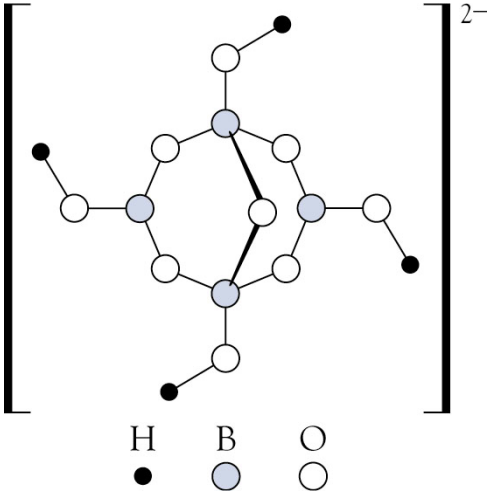
\includegraphics[width=0.5\textwidth]{figures/k13s293Borax.png}
\end{flashcard}

\begin{flashcard}[Struktur]{Tegn strukturen af peroxoborationen}
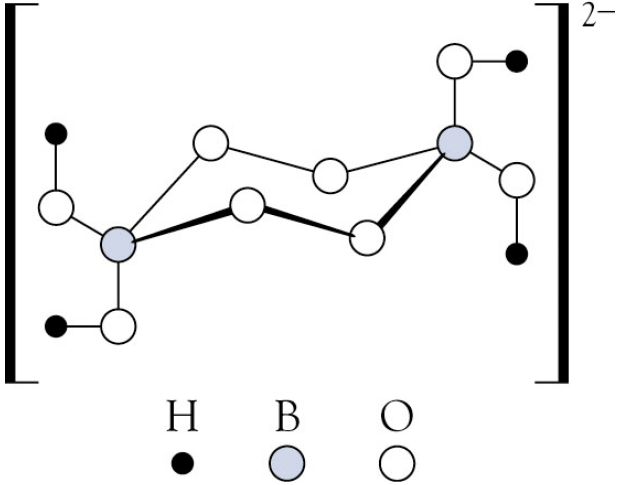
\includegraphics[width=0.5\textwidth]{figures/k13s293Peroxoborat.png}
\end{flashcard}

\begin{flashcard}[Fremstilling]{Opskriv reaktionen for fremstilling af peroxoborationen}
\ce{[B4O5(OH)4]^{2-} + 4H2O2 + 2OH- -> 2[B2(O2)2(OH)4]^{2-} + 3H2O}
\end{flashcard}

\begin{flashcard}[Fremstilling]{Opskriv reaktionen for fremstilling af borcarbid samt reaktionen for fremstilling af titaniumborid}
\ce{2B2O3 + 7C ->[\text{$\Delta$}] B4C + 6CO}\\ \vspace{7pt}
\ce{2TiO2 + B4C + 3C ->[\text{$\Delta$}] 2TiB2 + 4CO}
\end{flashcard}

\begin{flashcard}[Struktur]{Tegn strukturen af diboran}
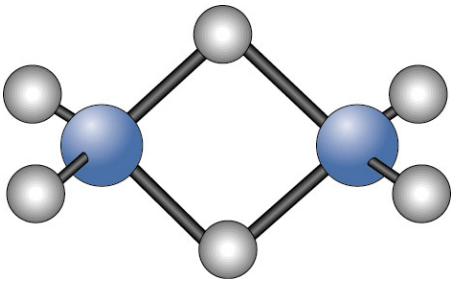
\includegraphics[width=0.5\textwidth]{figures/k13s295Diboran.png}
\end{flashcard}

\begin{flashcard}[Struktur]{Tegn strukturen af pentaboran(9)}
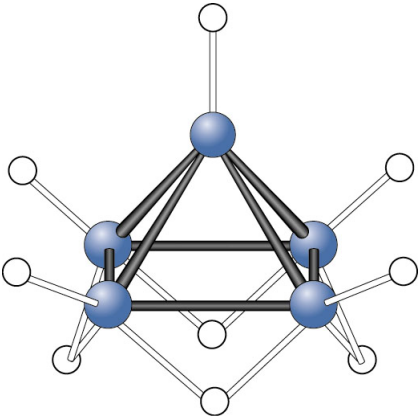
\includegraphics[width=0.5\textwidth]{figures/k13s296Pentaboran.png}
\end{flashcard}

\begin{flashcard}[Struktur]{Tegn strukturen af tetraboran(10)}
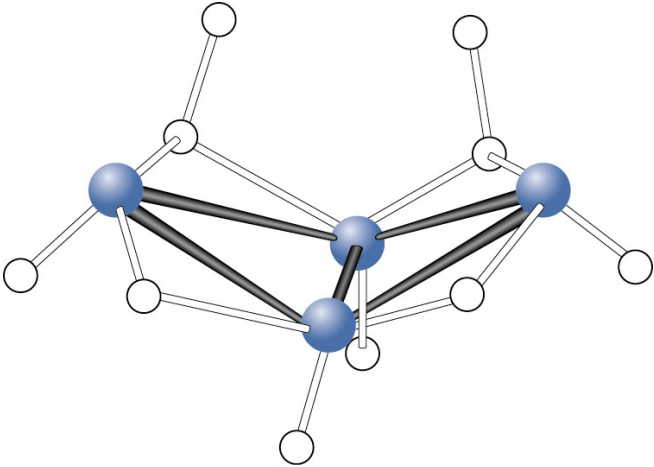
\includegraphics[width=0.7\textwidth]{figures/k13s296Tetraboran.png}
\end{flashcard}

\begin{flashcard}[Fremstilling]{Beskriv fremstillingen af diboran ved hj�lp af et reaktionsskema}
\begin{align*}
\ce{2\OX{rf1,\ox{+3,\ce{B}}}F3 + 6Na\OX{of1,\ox{-1,\ce{H}}} -> \OX{re1,\ox{-3,\ce{B2}}}\OX{oe1,\ox{+1,\ce{H6}}} + 6NaF}
\redox(of1,oe1){\small oxidation}
\redox(rf1,re1)[][-1]{\small reduktion}
\end{align*}
\end{flashcard}

\begin{flashcard}[Fremstilling]{Beskriv fremstillingen af tetraboran og pentaboran med reaktionsskemaer}
\ce{2B2H6 -> B4H10 + H2} \\ \vspace{7pt}
\ce{B4H10 + B2H6 -> 2B5H11 + 2H2}
\end{flashcard}

\begin{flashcard}[Reaktion]{Opskriv diborans reaktion med oxygen og vand}
\ce{B2H6 + 3O2 -> B2O3 + 3H2O}\\ \vspace{7pt}
\ce{B2H6 + 6H2O -> 2H3BO3 +6H2}
\end{flashcard}

\begin{flashcard}[Fremstilling]{Opskriv reaktionen for fremstilling af natriumborhydrid}
\ce{B2H6 + 2NaH -> 2NaBH4}
\end{flashcard}

\begin{flashcard}[Egenskab]{Aluminium metal er amfotert. Opskriv dets reaktion med syre henholdsvis base}
\ce{2Al + 6H+ + 6H2O -> 2[Al(OH2)6]^{3+} + 3H2}\\ \vspace{7pt}
\ce{2Al + 2OH- + 6H2O -> 2[Al(OH)4]- + 3H2}
\end{flashcard}

\begin{flashcard}[Egenskab]{Aluminium(III) i vandig opl�sning er en svag syre p� linje med eddikesyre. Opskriv reaktionen med vand}
\ce{[Al(OH2)6]^{3+} + H2O -> [Al(OH2)5(OH)]^{2+} + H3O+}
\end{flashcard}

\begin{flashcard}[Fremstilling]{Beskriv den industrielle fremstilling af aluminium metal med reaktionsskemaer}
\ce{Al2O3 + 2OH- + 3H2O -> 2[Al(OH)4]-}\\
\ce{2[Al(OH)4]- -> Al2O3\cdot 3H2O(s) + 2OH-}\\
\ce{Al2O3\cdot 3H2O ->[\text{$\Delta$}] Al2O3 + 3H2O}\\
Herefter f�lger elektrolyse af smeltet aluminiumoxid i cryolit
\end{flashcard}

\begin{flashcard}[Fremstilling]{Beskriv den industrielle fremstilling af cryolit med reaktionsskemaer}
\ce{3SiF4 + 2H2O -> 2H2SiF6 + SiO2}\\
\ce{H2SiF6 + 6NH3 + 2H2O -> 6NH4F + SiO2}\\ \vspace{7pt}
\ce{6NH4F + Na[Al(OH)4] + 2NaOH -> Na3AlF6 + 6NH3 + 6H2O}
\end{flashcard}

\begin{flashcard}[Struktur]{Hvilken struktur har \ce{MgAl2O4} henholdsvis \ce{Fe3O4}?}
\ce{MgAl2O4} er en spinel mens \ce{Fe3O4} er en invers spinel
\end{flashcard}
\cardfrontfoot{Kapitel 14}

\begin{flashcard}[Egenskab]{Opskriv 3 ioniske, 2 covalente og 2 metalliske carbider}
Ioniske: \ce{Na2C2}, \ce{Be2C} og \ce{Al4C3}\\ \vspace{7pt}
Covalente: \ce{SiC} og \ce{B4C}\\ \vspace{7pt}
Metalliske: \ce{WC} og \ce{Fe3C}
\end{flashcard}

\begin{flashcard}[Anvendelse]{Angiv en anvendelse af \ce{Na2C2}}
\ce{Na2C2 + 2H2O -> 2NaOH + C2H2}
\end{flashcard}

\begin{flashcard}[Fremstilling]{Angiv med reaktionsskema en metode til at fremstille carbonmonoxid i laboratoriet}
\ce{HCOOH + H2SO4(l) -> CO + H2O + H2SO4(aq)}
\end{flashcard}

\begin{flashcard}[Fremstilling]{Angiv med reaktionsskema hvordan man kan fremstille methanol og propanal ud fra bl.a. carbonmonoxid}
\ce{CO + 2H2 -> CH3OH} \\ \vspace{7pt}
\ce{CO + C2H4 + H2 -> C2H5CHO}
\end{flashcard}

\begin{flashcard}[Anvendelse]{Hvordan kan man unders�ge om der er carbondioxid i en gasstr�m?}
Man kan lede str�mmen gennem en opl�sning af  \ce{Ba(OH)2} eller \ce{Ca(OH)2}. Testen er positiv hvis der opst�r et bundfald.
\end{flashcard}

\begin{flashcard}[Reaktion]{Beskriv med reaktionsskema hvad der sker n�r man varmer f�lgende faste carbonater op:\\ \vspace{7pt}
\ce{CaCO3}, \ce{Ag2CO3}, \ce{(NH4)2CO3} og \ce{NaHCO3}
}
\ce{CaCO3 ->[\text{$\Delta$}] CaO + CO2}\\ \vspace{7pt}
\ce{Ag2CO3 ->[\text{$\Delta$}] Ag2O + CO2}\\
\ce{Ag2O ->[\text{$\Delta$}] 2Ag + $\frac{1}{2}$O2}\\ \vspace{7pt}
\ce{(NH4)2CO3 ->[\text{$\Delta$}] 2NH3 + H2O + CO2}\\ \vspace{7pt}
\ce{2NaHCO3 ->[\text{$\Delta$}] Na2CO3 + H2O + CO2}
\end{flashcard}

\begin{flashcard}[Fremstilling]{Beskriv med reaktionsskema hvordan man fremstiller carbondisulfid industrielt}
\ce{CH4 + 4S(l) ->[\text{$\Delta$}] CS2 + 2H2S}
\end{flashcard}

\begin{flashcard}[Fremstilling]{Opskriv to metoder til at producere \ce{CCl4}}
\begin{itemize}
\item \ce{CS2 + 3Cl2 ->[\text{$\rm FeCl_{3}/\Delta$}] CCl4 + S2Cl2}\\
\ce{CS2 + 2S2Cl2 ->[\text{$\Delta$}] CCl4 + 6S}
\item \ce{CH4 + 4Cl2 -> CCl4 + 4HCl}
 \end{itemize}
\end{flashcard}

\begin{flashcard}[Fremstilling]{Angiv to industrielle metoder til at fremstille bl�syre}
\ce{CH4 + NH3 ->[\text{$\rm Pt/1200\,^{\circ}{\rm C}$}] HCN + 3H2}\\ \vspace{7pt}
\ce{2CH4 + 2NH3 + 3O2 ->[\text{$\rm Pt/Rh/1100\,^{\circ}{\rm C}$}] 2HCN + 6H2O}
\end{flashcard}

\begin{flashcard}[Fremstilling]{Opskriv hvordan man fremstiller silicium industrielt}
\ce{SiO2 + 2C ->[\text{$\Delta$}] Si(l) + 2CO}
\end{flashcard}

\begin{flashcard}[Fremstilling]{Opskriv to metoder til at oprense silicium industrielt}
F�lgende ligev�gt kan bruges til at destillere silicium. Ligev�gten er forskudt med h�jre ved ca $300\,^{\circ}{\rm C}$ og mod venstre ved $1000\,^{\circ}{\rm C}$.\\
\ce{Si + 3HCl <=> SiHCl3(g) + H2}\\ \vspace{7pt}
En alternativ metode er zone-refining:
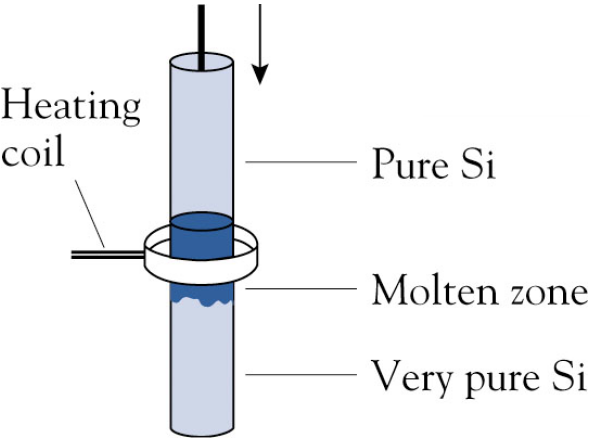
\includegraphics[width=0.37\textwidth]{figures/k14s340ZoneRefining.png}
\end{flashcard}

\begin{flashcard}[Reaktion]{Opskriv den kemiske formel for to kemikalier som kan reagere med glas samt deres reaktion}
Der er tale om \ce{HF} og \ce{NaOH}\\ \vspace{7pt}
\ce{SiO2 + 6HF -> SiF6^{2-} + 2H+ + 2H2O}\\ \vspace{7pt}
\ce{SiO2 + 2NaOH ->[\text{$\Delta$}] Na2SiO3 + H2O}
\end{flashcard}

\begin{flashcard}[Egenskab]{Opskriv de fire typer glas der er omtalt i bogen og angiv fordele ved hver af dem}
\begin{itemize}
\item Soda-lime\\Billigt
\item Borosilicate\\Kan klare store temperaturudsving
\item Lead\\Absorberer radioaktiv str�ling
\item Quartz\\Er ogs� gennemsigtigt i UV omr�det
\end{itemize}
\end{flashcard}

\begin{flashcard}[Fremstilling]{Angiv med reaktionsskema hvordan man kan fremstille natriumsilicat}
\ce{SiO2 + 2Na2CO3(l) ->[\text{$\Delta$}] Na4SiO4 + 2CO2}
\end{flashcard}

\begin{flashcard}[Struktur]{Tegn strukturen af pyrosilicationen}
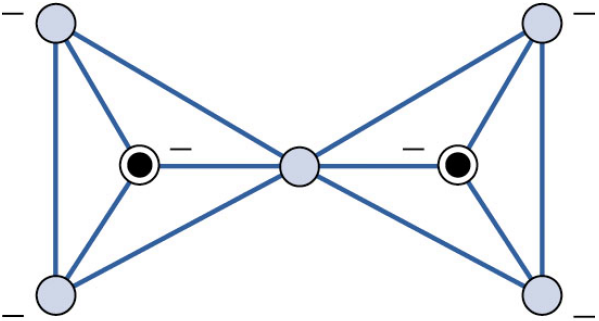
\includegraphics[width=0.5\textwidth]{figures/k14s344Pyrosilicate.png}
\end{flashcard}

\begin{flashcard}[Reaktion]{Angiv reaktionen mellem silicationen og syre}
\ce{2SiO4^{4-} + 2H+ -> Si2O7^{6-} + H2O}
\end{flashcard}

\begin{flashcard}[Struktur]{Angiv de kemiske formler for hvid og bl� asbest og angiv hvilken der er farligst}
Hvid asbest: \ce{Mg3(Si2O5)(OH)4}\\ \vspace{7pt}

Bl� asbest: \ce{Na2Fe5(Si4O11)2(OH)2} (farligst)
\end{flashcard}

\begin{flashcard}[Fremstilling]{Angiv hvordan silikone laves ved hj�lp af reaktionsskemaer samt strukturen af silikone}
\ce{2CH3Cl + Si ->[\text{$\Delta$}] (CH3)2SiCl2}\\
\ce{(CH3)2SiCl2 + 2H2O -> (CH3)2(Si(OH)2 + 2HCl}\\
\ce{$n$(CH3)2Si(OH)2 -> [-O-Si(CH3)2-]_{$n$} + H2O}\\ \vspace{7pt}
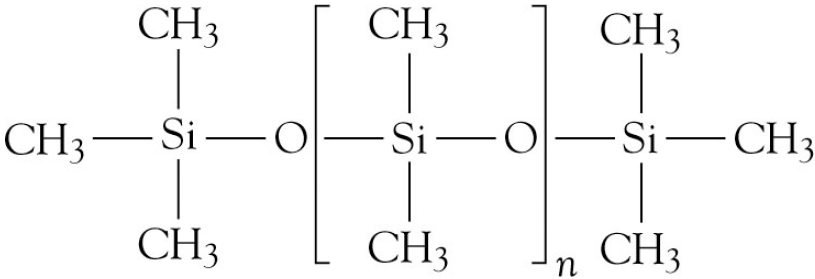
\includegraphics[width=0.9\textwidth]{figures/k14s349Silikone.png}
\end{flashcard}

\begin{flashcard}[Reaktion]{Angiv tin(II)oxids reaktion med syre henholdsvis base}
\ce{SnO + 2HCl -> SnCl2 + H2O}\\ \vspace{7pt}
\ce{SnO + NaOH + H2O -> Na+ + [Sn(OH)3]-}
\end{flashcard}

\begin{flashcard}[Fremstilling]{Angiv den prim�re kilde af bly i naturen samt hvordan man udvinder bly fra denne}
Den prim�re naturlige kilde er \ce{PbS}\\ \vspace{7pt}
\ce{2PbS + 3O2 ->[\text{$\Delta$}] 2PbO + 2SO2}\\
\ce{PbO + C ->[\text{$\Delta$}] Pb + CO}
\end{flashcard}

\begin{flashcard}[Reaktion]{Angiv med reaktionsskema hvorledes \ce{PbCl4} dekomponerer}
\begin{align*}
\ce{\OX{rf1,\ox{+4,\ce{Pb}}}\OX{of1,\ox{-1,\ce{Cl4}}} -> \OX{re1,\ox{2,\ce{Pb}}} Cl2 + \OX{oe1,\ox{0,\ce{Cl2}}}}
\redox(of1,oe1){\small oxidation}
\redox(rf1,re1)[][-1]{\small reduktion}
\end{align*}
\end{flashcard}
\cardfrontfoot{Kapitel 15}

\begin{flashcard}[Egenskab]{Hvordan fremst�r grundstofferne i 5. hovedgruppe ved SATP?}
Nitrogen er en farvel�s gas. Fosfor er en hvis voks-agtig substans. De resterende er skr�blige metaller.
\end{flashcard}

\begin{flashcard}[Teori]{Angiv de specier der har tendens til at disproportionere i sur opl�sning\\
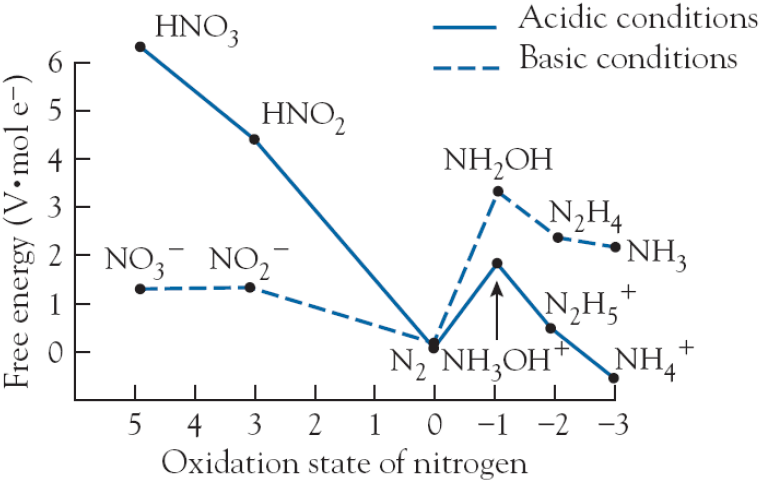
\includegraphics[width=0.55\textwidth]{figures/k15s368FrostDiagram.png}
}
\ce{HNO2} samt \ce{NH3OH+}
\end{flashcard}

\begin{flashcard}[Fremstilling]{Angiv hvordan ammoniak kan fremstilles i laboratoriet}
\ce{NH4Cl + NaOH -> NH3(g) + NaCl}
\end{flashcard}

\begin{flashcard}[Fremstilling]{Opskriv hvordan ammoniak fremstilles industrielt}
\ce{CH4 + H2O -> CO + 3H2}\\
\ce{ZnO + H2S -> ZnS + 2H2O}\\
\ce{Ch4 + $\frac{1}{2}$O2 + 2N2 -> CO + 2H2 + 2N2}\\
\ce{CO + H2O <=> CO + H2}\\
\ce{CO2 + K2CO3 + H2O <=> 2KHCO3}\\
\ce{ N_{2} + 3H_{2} <=> 2NH_{3}}\\ \vspace{7pt}
ved et tryk p� 100-1000 atm og en temperatur p� 400-500$\,^{\circ}{\rm C}$
\end{flashcard}

\begin{flashcard}[Egenskab]{Reagerer hydrazin alkalisk eller neutralt?}
Alkalisk\\ \vspace{7pt}
\ce{N2H4 + H3O+ -> N2H5+ + H2O}
\end{flashcard}

\begin{flashcard}[Egenskab]{Angiv hvordan hydrazin kan anvendes som reduktionsmiddel}
\ce{N2H4 + 2I2 -> 4HI + N2}\\ \vspace{7pt}
\ce{N2H4 + 2Cu^{2+} -> 2Cu + N2 + 4H+}
\end{flashcard}

\begin{flashcard}[Struktur]{Tegn hydrazin}
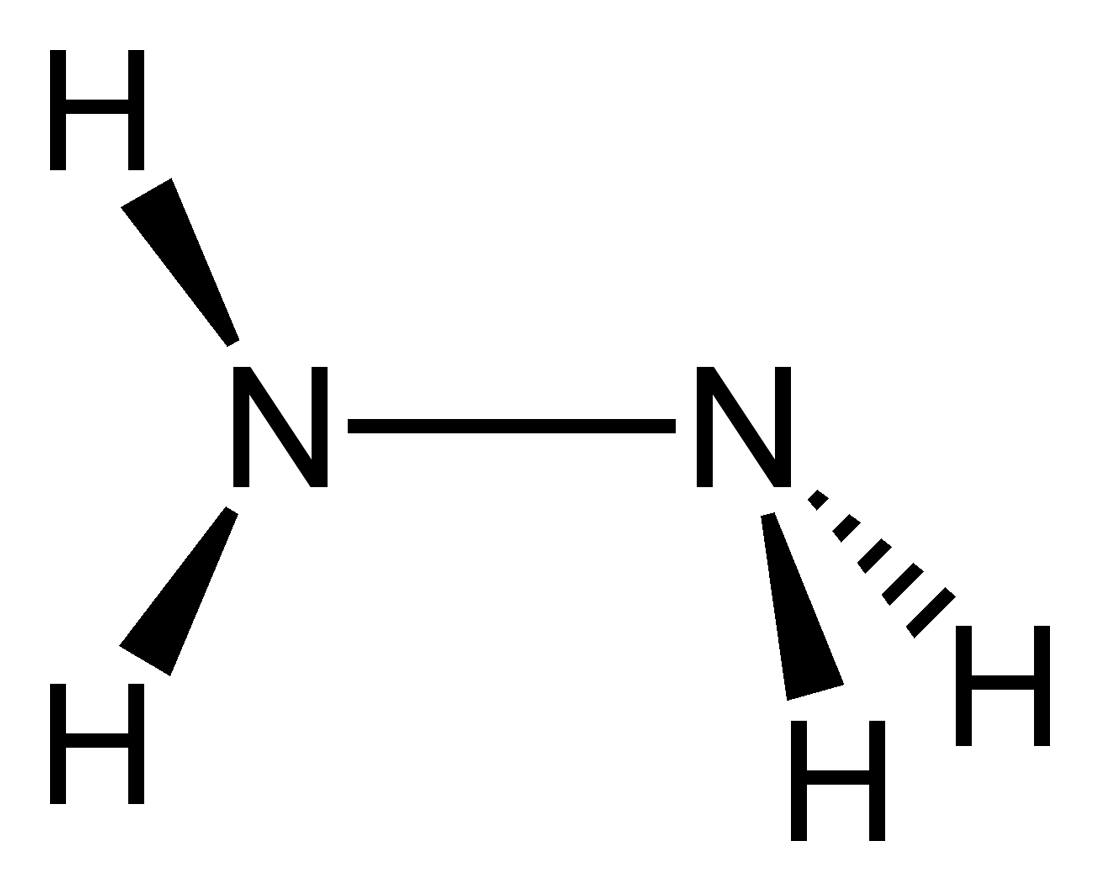
\includegraphics[width=0.55\textwidth]{figures/Hydrazin.png}
\end{flashcard}

\begin{flashcard}[Reaktion]{Angiv hvordan hydrogenazid dekomponerer}
\ce{2HN3 -> H2 + 3N2}
\end{flashcard}

\begin{flashcard}[Anvendelse]{Forklar hvordan en airbag virker ved hj�lp af reaktionsligninger}
\ce{2NaN3 ->[\text{$\Delta$}] 2Na(l) + 3N2}\\
\ce{10Na(l) + 2KNO3 -> K2O + 5Na2O + N2}\\
\ce{2K2O + SiO2 -> K4SiO4}\\
\ce{2Na2O + SiO2 -> Na4SiO4}
\end{flashcard}

\begin{flashcard}[Reaktion]{Angiv hvordan f�lgende forbindelser dekomponerer ved opvarmning\\
\ce{NH4NO2}, \ce{NH4NO3} samt \ce{(NH4)2Cr2O7}
}
\ce{NH4NO2 ->[\text{$\Delta$}] N2 + 2H2O}\\ \vspace{7pt}
\ce{NH4NO3 ->[\text{$\Delta$}] N2O + 2H2O}\\ \vspace{7pt}
\ce{(NH4)2Cr2O7 ->[\text{$\Delta$}] N2 + Cr2O3 + 4H2O}
\end{flashcard}

\begin{flashcard}[Reaktion]{Angiv en metode til at producere lattergas}
\ce{NH4NO3 ->[\ce{H+}] N2O + 2H2O}
\end{flashcard}

\begin{flashcard}[Reaktion]{Angiv en metode til at producere nitrogenmonoxid}
\ce{3Cu + 8HNO3 -> 3Cu(NO3)2 + 4H2O + 2NO}
\end{flashcard}

\begin{flashcard}[Reaktion]{Angiv en metode til at producere \ce{N2O3}}
\ce{NO + NO2 -> N2O3(l)}
\end{flashcard}

\begin{flashcard}[Reaktion]{Angiv reaktionen mellem \ce{N2O3} og vand}
\ce{N2O3 + H2O -> 2HNO2}
\end{flashcard}

\begin{flashcard}[Struktur]{Tegn dinitrogentrioxid}
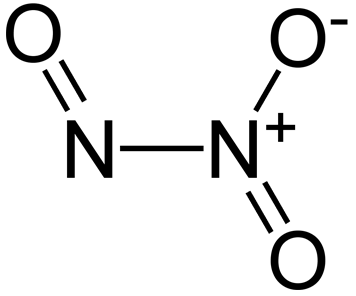
\includegraphics[width=0.55\textwidth]{figures/Dinitrogentrioxid.png}
\end{flashcard}

\begin{flashcard}[Reaktion]{Angiv to metoder til at producere nitrogendioxid}
\ce{Cu + 4HNO3 -> Cu(NO3)2 + 2H2O + 2NO2}\\ \vspace{7pt}
\ce{Cu(NO3)2 ->[\text{$\Delta$}] CuO + 2NO2 + $\frac{1}{2}$O2}
\end{flashcard}

\begin{flashcard}[Reaktion]{Angiv reaktionen mellem nitrogendioxid og vand}
\ce{2NO2 + H2O <=> HNO3 + HNO2}
\end{flashcard}

\begin{flashcard}[Struktur]{Tegn nitrogendioxid}
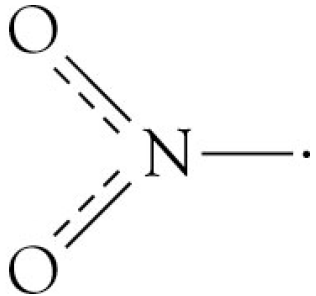
\includegraphics[width=0.3\textwidth]{figures/k15s383Nitrogendioxid.png}
\end{flashcard}

\begin{flashcard}[Struktur]{Tegn dinitrogentetroxid}
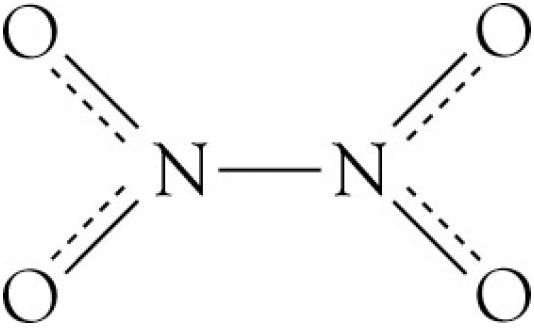
\includegraphics[width=0.5\textwidth]{figures/k15s383Dinitrogentetroxid.png}
\end{flashcard}

\begin{flashcard}[Struktur]{Tegn dinitrogenpentoxid}
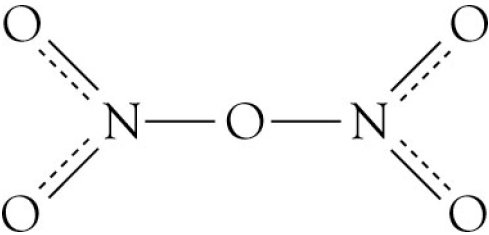
\includegraphics[width=0.5\textwidth]{figures/k15s383Dinitrogenpentoxid.png}
\end{flashcard}

\begin{flashcard}[Struktur]{Tegn nitrat}
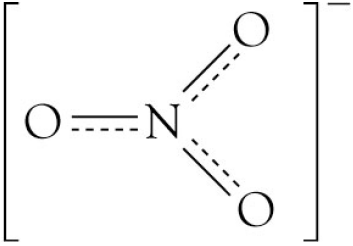
\includegraphics[width=0.5\textwidth]{figures/k15s383Nitrat.png}
\end{flashcard}

\begin{flashcard}[Struktur]{Tegn nitrit}
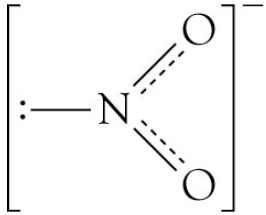
\includegraphics[width=0.5\textwidth]{figures/k15s385Nitrit.png}
\end{flashcard}

\begin{flashcard}[Fremstilling]{Angiv med reaktionsligning hvordan man kan fremstille salpetersyrling i laboratoriet}
\ce{Ba(NO2)2 + H2SO4 -> BaSO4(s) + 2HNO2}
\end{flashcard}

\begin{flashcard}[Reaktion]{Angiv med reaktionsligning hvordan salpetersyrling disproportionerer}
\begin{align*}
\ce{3H\OX{d,\ox{+3,\ce{N}}}O2 -> H\OX{oe1,\ox{5,\ce{N}}}O3 + 2\OX{re1,\ox{+2,\ce{N}}}O}
\redox(d,oe1){\small oxidation}
\redox(d,re1)[][-1]{\small reduktion}
\end{align*}\\ \vspace{15pt}
(\ce{2NO + O2 -> 2NO2})
\end{flashcard}

\begin{flashcard}[Fremstilling]{Opskriv hvordan man producerer salpetersyre industrielt via. Ostwald-processen}
\ce{4NH3 + 5O2 -> 4NO + 6H2O}\\
\ce{2NO + O2 -> 2NO2}\\
\ce{3NO2 + H2O -> 2HNO3 + NO}
\end{flashcard}

\begin{flashcard}[Anvendelse]{Angiv den eksoterme reaktion der finder sted i en cold pack}
\ce{NH4NO3(s) -> NH4+ + NO3-}
\end{flashcard}

\begin{flashcard}[Struktur]{Tegn strukturen af hvid henholdsvis r�d fosfor}
Hvid:\\
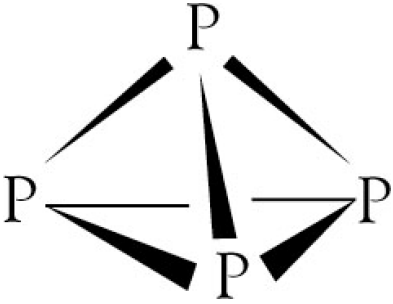
\includegraphics[width=0.2\textwidth]{figures/k15s390HvidP.png}\\
R�d:\\
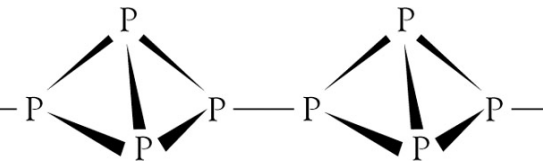
\includegraphics[width=0.6\textwidth]{figures/k15s390RodP.png}
\end{flashcard}

\begin{flashcard}[Reaktion]{Hvad sker der med hvid fosfor der uds�ttes for UV lys?}
Det omdannes til dens allotrop, r�d fosfor
\end{flashcard}

\begin{flashcard}[Reaktion]{Hvorfor skal hvid fosfor opbevares under vand?}
Fordi det reagerer med atmosf�rens oxygen\\
\ce{P4 + 5O2 -> P4O10}
\end{flashcard}

\begin{flashcard}[Fremstilling]{Hvordan udvindes fosfor industrielt?}
\ce{2Ca3(PO4)2 + 10CO ->[\text{$\Delta$}] 6CaO + 10CO2 + P4(g)}\\
\ce{CO2 + C -> 2CO} \\
\ce{CaO + SiO2 ->[\text{$\Delta$}] CaSiO3(l)}\\ \vspace{7pt}
Reaktionerne foreg�r ved $\rm 1500\,^{\circ}{\rm C}$.
\end{flashcard}

\begin{flashcard}[Fremstilling]{Hvordan fremstilles phosphin?}
\ce{Ca3P2 + 6H2O(s) -> 2PH3 + 3Ca(OH)2}
\end{flashcard}

\begin{flashcard}[Reaktion]{Opskriv reaktionerne hvorved de to oxider af fosfor dannes}
\ce{P4 + 3O2 -> P4O6}\\ \vspace{7pt}
\ce{P4 + 5O2 -> P4O10}
\end{flashcard}

\begin{flashcard}[Struktur]{Tegn strukturen af \ce{P4O6}}
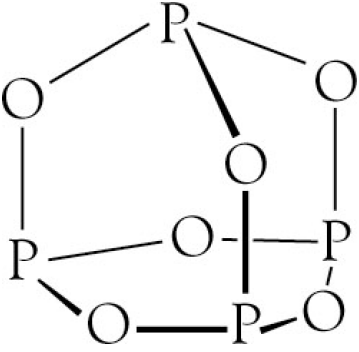
\includegraphics[width=0.4\textwidth]{figures/k15s393P4O6.png}
\end{flashcard}

\begin{flashcard}[Struktur]{Tegn strukturen af \ce{P4O10}}
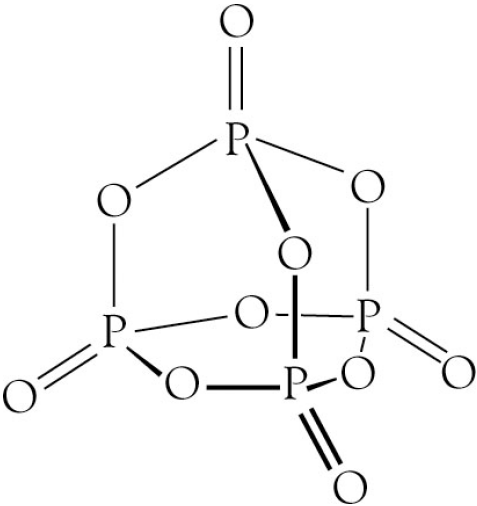
\includegraphics[width=0.4\textwidth]{figures/k15s394P4O10.png}
\end{flashcard}

\begin{flashcard}[Reaktion]{Angiv reaktionen mellem \ce{P4O10} og vand}
\ce{P4O10 + 6H2O + 4H3PO4}
\end{flashcard}

\begin{flashcard}[Reaktion]{Opskriv reaktionligninger for hvordan man danner de to chlorider af fosfor}
\ce{P4 + 6Cl2 -> 4PCl3}\\ \vspace{7pt}
\ce{P4 + 10Cl2 -> 4PCl5}
\end{flashcard}

\begin{flashcard}[Reaktion]{Angiv phosphortrichlorids henholdsvis phosphorpentachlorids reaktion med vand}
\ce{PCl3 + H2O -> H3PO3 + 3HCl}\\ \vspace{7pt}
\ce{PCl5 + H2O -> POCl3 + 2HCl}\\
\ce{POCl3 + 3H2O -> H3PO4 + 3HCl}
\end{flashcard}

\begin{flashcard}[Fremstilling]{Angiv med reaktionsskema hvorledes \ce{POCl3} fremstilles}
\ce{2PCl3 + O2 -> 2POCl3}
\end{flashcard}

\begin{flashcard}[Struktur]{Tegn \ce{H3PO4}, \ce{H3PO3} samt \ce{H3PO2}}
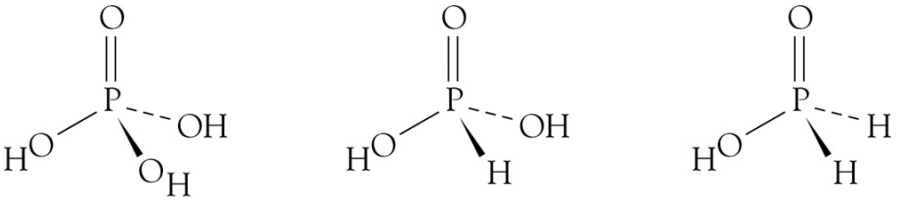
\includegraphics[width=0.9\textwidth]{figures/k15s395POxyAcids.png}
\end{flashcard}

\begin{flashcard}[Fremstilling]{Angiv hvordan fosforsyre fremstilles ved v�dprocessen}
\ce{Ca3(PO4)2 + 3H2SO4 -> 3CaSO4(s) + 2H3PO4}
\end{flashcard}

\begin{flashcard}[Struktur]{Angiv strukturen af kondensationsproduktet der f�s ved opvarmning af fosforsyre}
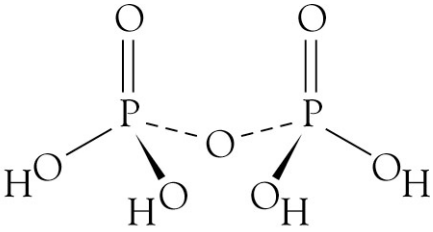
\includegraphics[width=0.6\textwidth]{figures/k15s396H4P2O7.png}
\end{flashcard}

\begin{flashcard}[Fremstilling]{Angiv med reaktionsskema hvordan calciumfosfat kan bearbejdes s� det kan bruges som g�dning}
\ce{Ca3(PO4)2(s) + 2H2SO4 -> Ca(H2PO4)2(s) + 2CaSO4(s)}
\end{flashcard}
\cardfrontfoot{Kapitel 16}

\begin{flashcard}[Fremstilling]{Angiv 2 metoder til at fremstille oxygen i laboratoriet}
\ce{2KClO3 ->[\text{$\rm MnO2/\Delta$}] 2KCl + 3O2}\\ \vspace{7pt}
\ce{2H2O2 ->[\text{$\rm MnO2$}] 2H2O + O2}
\end{flashcard}

\begin{flashcard}[Fremstilling]{Angiv hvordan man kan fremstille diamagnetisk \ce{O2}}
\ce{H2O2 + ClO- -> O2 + H2O + Cl-}
\end{flashcard}

\begin{flashcard}[Fremstilling]{Angiv hvordan man kan fremstille ozon}
\ce{3O2 -> 2O3}\\
ved p�f�ring af en sp�nding p� 10-20kV
\end{flashcard}

\begin{flashcard}[Reaktion]{Angiv produktet af reaktion mellem f�lgende forbindelser og ozon: \ce{NO2}, \ce{CN-} samt \ce{PbS}}
\ce{2NO2 + O3 -> N2O5 + O2} \\ \vspace{7pt}
\ce{CN- + O3 -> OCN- + O2} \\ \vspace{7pt}
\ce{PbS + 4O3 -> PbSO4 + 4O2}
\end{flashcard}

\begin{flashcard}[Egenskab]{Kategoriser disse metaloxider som enten: meget basiske, basiske, amfotere eller sure\\
\ce{Na2O}, \ce{CaO}, \ce{MnO}, \ce{Al2O3}, \ce{Cr2O3}, \ce{SnO2}, \ce{V2O5}, \ce{CrO3} samt \ce{Mn2O7}
}
Meget basisk: \ce{Na2O}\\
Basisk: \ce{CaO} og \ce{MnO}\\
Amfoter: \ce{Al2O3}, \ce{Cr2O3}, \ce{SnO2} og \ce{V2O5}\\
Sure: \ce{CrO3} og \ce{Mn2O7}
\end{flashcard}

\begin{flashcard}[Egenskab]{Kategoriser disse ikke-metaloxider som enten: neutrale, sure eller meget sure\\
\ce{N2O}, \ce{CO}, \ce{N2O3}, \ce{NO2}, \ce{CO2}, \ce{SO2}, \ce{N2O5}, \ce{SO3} samt \ce{Cl2O7}
}
Neutrale: \ce{N2O} og \ce{CO}\\
Sure: \ce{N2O3}, \ce{NO2}, \ce{CO2} og \ce{SO2}\\
Meget sure: \ce{N2O5}, \ce{SO3} og \ce{Cl2O7}
\end{flashcard}

\begin{flashcard}[Fremstilling]{Angiv hvordan hydrogenperoxid kan fremstilles i laboratoriet}
\ce{Na2O2 + 2H2O -> 2NaOH + H2O2}
\end{flashcard}

\begin{flashcard}[Egenskab]{Hydrogenperoxid har tendens til at disproportionere. Opskriv reaktionen}
\ce{2H2O2 -> 2H2O + O2}
\end{flashcard}

\begin{flashcard}[Struktur]{Tegn strukturen af \ce{S6}}
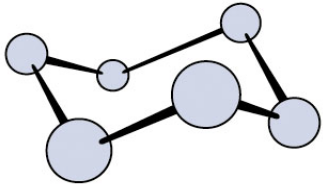
\includegraphics[width=0.6\textwidth]{figures/k16s428S6.png}
\end{flashcard}

\begin{flashcard}[Struktur]{Tegn strukturen af \ce{S8}}
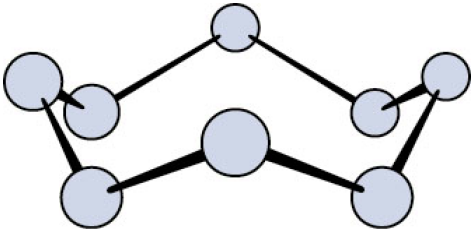
\includegraphics[width=0.6\textwidth]{figures/k16s427S8.png}
\end{flashcard}

\begin{flashcard}[Struktur]{Tegn strukturen af \ce{S12}}
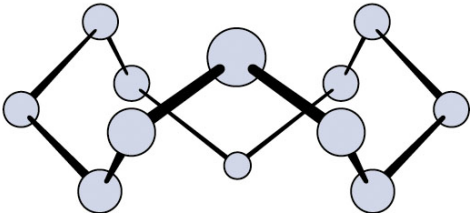
\includegraphics[width=0.7\textwidth]{figures/k16s428S12.png}
\end{flashcard}

\begin{flashcard}[Fremstilling]{Opskriv hvordan man kan fremstille \ce{S6}}
\ce{6Na2S2O3 + 12HCl -> S6(s) + 6SO2 + 12NaCl + 6H2O}
\end{flashcard}

\begin{flashcard}[Fremstilling]{Opskriv hvordan man kan fremstille \ce{S12}}
\ce{H2S8 + S4Cl2 -> S12(s) + 2HCl(g)}
\end{flashcard}

\begin{flashcard}[Fremstilling]{Opskriv reaktionsligninger der beskriver Claus processen}
\ce{2H2S + 3O2 -> 2SO2 + 2H2O}\\
\ce{4H2S + 2SO2 -> 6S(s) + 4H2O}
\end{flashcard}

\begin{flashcard}[Fremstilling]{Angiv hvordan man kan udvinde svovl fra pyrit}
\ce{FeS2 ->[\text{$\Delta$}] FeS + S(s)}
\end{flashcard}

\begin{flashcard}[Reaktion]{Hvordan kan man p�vise sulfid i en vandig opl�sning?}
\ce{Pb(CH3COO)2 + H2S(g) -> PbS + 2CH3COOH}\\ \vspace{7pt}
Blyacetat er farvel�st. Ved reaktion fremkommer sort bly(II)sulfid
\end{flashcard}

\begin{flashcard}[Reaktion]{Hvordan kan man p�vise \ce{SO2} i en vandig opl�sning?}
\ce{Cr2O7^{2-} + 3SO2 + 2H+ -> 2Cr^{3+} + 3SO4^{2-} + H2O}\\ \vspace{7pt}
Dichromat er orange/gult. Ved reaktion skifter opl�sningen farve til gr�n pga. chrom(III) ioner
\end{flashcard}

\begin{flashcard}[Reaktion]{Hvordan kan kraftv�rker oplagre \ce{SO2}?}
\ce{2CaO + 2SO2 + O2 ->[\text{$\Delta$}] 2CaSO4}
\end{flashcard}

\begin{flashcard}[Fremstilling]{Opskriv reaktionsligninger der beskriver trinnene i den industrielle syntese af svovlsyre}
\ce{S + O2 ->[\text{$\Delta$}] SO2}\\
\ce{2SO2 + O2 ->[\text{$\rm V_{2}O_{5}/\Delta$}] 2SO3}\\
\ce{SO3 + H2SO4 -> H2S2O7}\\
\ce{H2S2O7 + H2O -> 2H2SO4}
\end{flashcard}

\begin{flashcard}[Struktur]{Tegn strukturen af \ce{H2SO4}}
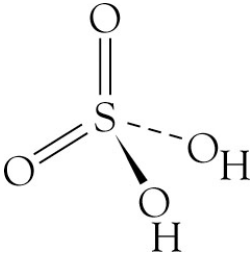
\includegraphics[width=0.4\textwidth]{figures/k16s438H2SO4.png}
\end{flashcard}

\begin{flashcard}[Struktur]{Tegn strukturen af \ce{H2S2O7}}
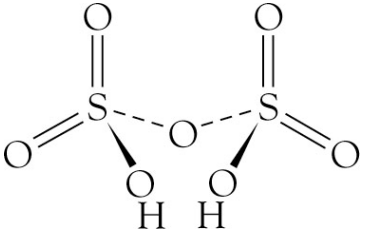
\includegraphics[width=0.7\textwidth]{figures/k16s439H2S2O7.png}
\end{flashcard}

\begin{flashcard}[Reaktion]{Hvad sker der hvis man varmer svovlsyre?}
\ce{2H2SO4 ->[\text{$\Delta$}] 2SO2 + 2H2O + O2}
\end{flashcard}

\begin{flashcard}[Fremstilling]{Angiv hvordan man kan fremstille thiosulfationen}
\ce{SO3^{2-} + S -> S2O3^{2-}}
\end{flashcard}

\begin{flashcard}[Struktur]{Tegn thiosulfationen}
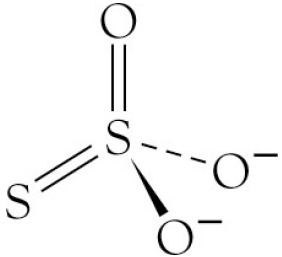
\includegraphics[width=0.5\textwidth]{figures/k16s442S2O32-.png}
\end{flashcard}

\begin{flashcard}[Struktur]{Tegn produktet af elektrolytisk oxidation af thiosulfationen}
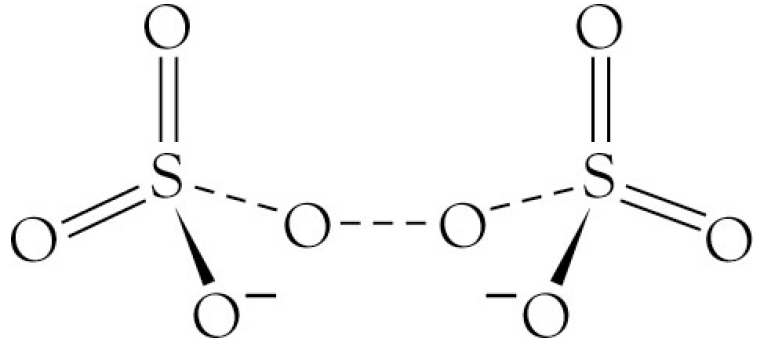
\includegraphics[width=0.7\textwidth]{figures/k16s443Peroxodisulfat.png}
\end{flashcard}

\begin{flashcard}[Fremstilling]{Angiv den simple reaktion for fremstilling af den inerte gas \ce{SF6}}
\ce{S(l) + 3F2(g) -> SF6(g)}
\end{flashcard}

\begin{flashcard}[Struktur]{Tegn strukturen af \ce{S2Cl2}}
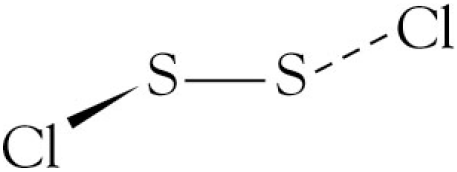
\includegraphics[width=0.7\textwidth]{figures/k16s444S2Cl2.png}
\end{flashcard}
\cardfrontfoot{Kapitel 17}

\begin{flashcard}[Egenskab]{Hvordan fremst�r halogenerne ved SATP?}
\ce{F2} fremst�r som en bleg gul gas og \ce{Cl2} som en bleg gr�n gas. \ce{Br2} er en r�dbrun visk�s v�ske. Iod fremst�r som glimtende sort-violette krystaller.
\end{flashcard}

\begin{flashcard}[Fremstilling]{Hvordan fremstilles \ce{F2}?}
Elektrolyse af kaliumfluorid
\end{flashcard}

\begin{flashcard}[Fremstilling]{Hvordan fremstilles \ce{UF6} industrielt?}
\ce{UO2 + 4HF -> UF4(s) + 2H2O}\\
\ce{UF4(s) + F2 -> UF6(g)}
\end{flashcard}

\begin{flashcard}[Fremstilling]{Hvordan produceres flussyre industrielt?}
\ce{CaF2 + H2SO4 -> 2HF(g) + CaSO4}
\end{flashcard}

\begin{flashcard}[Fremstilling]{Hvordan kan man fremstille chlorgas i laboratoriet og i industrien?}
I laboratoriet kan man n�jes med f�lgende\\
\ce{10HCl + 2MnO4- + 6H+ -> 5Cl2 + 2Mn^{2+} + 8H2O}\\ \vspace{7pt}
Industrielt produceres chlorgas som biprodukt ved elektrolyse af eksempelvis natriumchlorid opl�sning med henblik p� at producere natriummetal.
\end{flashcard}

\begin{flashcard}[Reaktion]{Angiv reaktionen mellem \ce{Cl2} og vand}
\ce{Cl2 + H2O -> H+ + Cl- + HClO}
\end{flashcard}

\begin{flashcard}[Fremstilling]{Hvordan fremstilles saltsyre industrielt?}
Saltsyre produceres hovedsagligt som biprodukt af andre synteser. Eksempelvis:\\
\ce{CH4 + 4Cl2 -> CCl4 + 4 HCl}
\end{flashcard}

\begin{flashcard}[Reaktion]{Hvordan fremstiller man jern(II)chlorid henholdsvis jern(III)chlorid?}
\ce{Fe + 2HCl -> FeCl2 + H2}\\ \vspace{7pt}
\ce{2Fe + 3Cl2 -> 2FeCl3}
\end{flashcard}

\begin{flashcard}[Reaktion]{Et af de 3 tungtopl�selige s�lvhalider g�r i opl�sning ved tils�tning af ammoniak. Hvilket?}
Chlorid\\ \vspace{7pt}
\ce{AgCl(s) + 2NH3 -> [Ag(NH3)2]+ + Cl-}
\end{flashcard}

\begin{flashcard}[Struktur]{Angiv struktueren af f�lgende forbindelser: Hypochlorsyrling, chlorsyrling, chlorsyre og perchlorsyre}
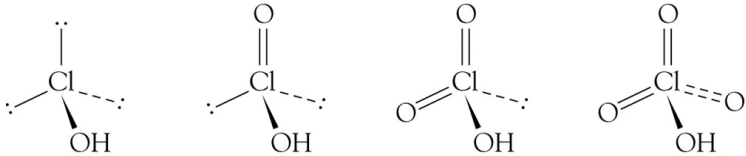
\includegraphics[width=\textwidth]{figures/k17s471Cl.png}
\end{flashcard}

\begin{flashcard}[Reaktion]{Angiv den reaktion der finder sted n�r chlorgas opl�ses i vand}
\ce{Cl2 + H2O <=> H+ + Cl- + HClO}
\end{flashcard}

\begin{flashcard}[Fremstilling]{Hvordan fremstilles perchlorat?}
\ce{3Cl2 + 6NaOH -> NaClO3 + 5NaCl(s) + 3H2O}\\ \vspace{7pt}
\ce{4KClO3(l) ->[\text{$\Delta$}] KCl(s) + 3KClO4(s)}
\end{flashcard}

\begin{flashcard}[Anvendelse]{Angiv reaktionen der finder sted n�r en faststof l�fteraket affyres}
\ce{6NH4ClO4 + 8Al -> 4Al2O3 + 3N2 + 3Cl2 + 12H2O(g)}
\end{flashcard}
\cardfrontfoot{Kapitel 18}

\begin{flashcard}[Struktur]{Tegn \ce{XeF2}, \ce{XeF4} og \ce{XeF6}}
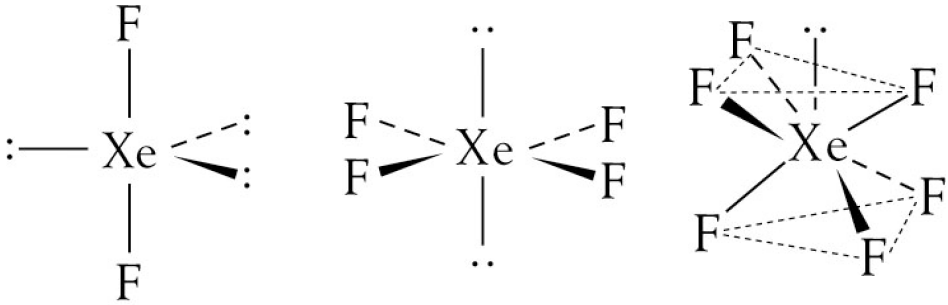
\includegraphics[width=1\textwidth]{figures/k18s493XeF.png}
\end{flashcard}

\begin{flashcard}[Struktur]{Tegn \ce{XeO3} og \ce{XeO4}}
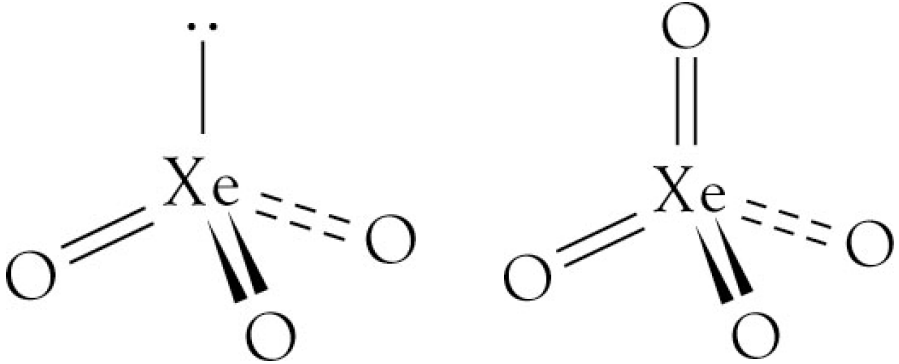
\includegraphics[width=0.8\textwidth]{figures/k18s494XeO.png}
\end{flashcard}
\end{document}